\qrchapter{https://forgottenpillar.com/rsc/en-fp-chapter4}{Revision of “Living Temple”}


\qrchapter{https://forgottenpillar.com/rsc/en-fp-chapter4}{Révision du “Temple Vivant”}


In \textit{Testimonies for the Church Containing Letters to Physicians and Ministers Instruction to Seventh-Day Adventists}, the tenth chapter, \textit{The Foundation of our Faith,} God gave valuable lessons on the development and consequences of Kellogg's theories. The broader and deeper meaning of these quotations can be understood when we are familiar with their historical context. Let us first take a brief look at the historical context of Kellogg's book, The \textit{Living Temple}.


Dans \textit{Témoignages pour l'Église contenant des lettres aux médecins et aux pasteurs - Instruction aux Adventistes du Septième Jour}, le dixième chapitre, \textit{Le Fondement de notre Foi,} Dieu a donné de précieuses leçons sur le développement et les conséquences des théories de Kellogg. La signification plus large et plus profonde de ces citations peut être comprise lorsque nous sommes familiers avec leur contexte historique. Examinons d'abord brièvement le contexte historique du livre de Kellogg, Le \textit{Temple Vivant}.


In a series of providence, God signified that “\textit{Living Temple}” should not be printed. One such event was the burning of Battle Creek's press building, just the night before it was to be printed. Finally, the book was printed elsewhere; it instigated a great crisis in the Seventh-day Adventist Church. On October 7, 1903, a annual meeting of the conference was held in Washington DC. Many Seventh-day Adventist church leaders were present, including Dr. Kellogg and his sympathizers. Major controversy was taking place over this book and the conflict was inevitable. Fortunately, on the brink of this escalating conflict, a letter from Sister White was delivered to the council. On Sunday, the letter fell upon the ears of all, to which there resounded many “amen's” and “halleluyah's”. It was a very tense and moving morning for the church that was on the verge of a split—to at last have concrete direction from the Lord's messenger:


Par une série de providences, Dieu a signifié que “\textit{Le Temple Vivant}” ne devait pas être imprimé. L'un de ces événements fut l'incendie du bâtiment de la presse de Battle Creek, la veille même de son impression. Finalement, le livre a été imprimé ailleurs; il a provoqué une grande crise dans l'Église Adventiste du Septième Jour. Le 7 octobre 1903, une réunion annuelle de la conférence s'est tenue à Washington DC. De nombreux dirigeants de l'Église Adventiste du Septième Jour étaient présents, y compris le Dr Kellogg et ses sympathisants. Une controverse majeure avait lieu au sujet de ce livre et le conflit était inévitable. Heureusement, au bord de ce conflit qui s'intensifiait, une lettre de Sœur White a été remise au conseil. Le dimanche, la lettre est parvenue aux oreilles de tous, ce qui a suscité de nombreux “amen” et “alléluia”. Ce fut une matinée très tendue et émouvante pour l'église qui était au bord de la division—pour enfin avoir une direction concrète de la messagère du Seigneur:


\begin{figure}[h]
    \centering
    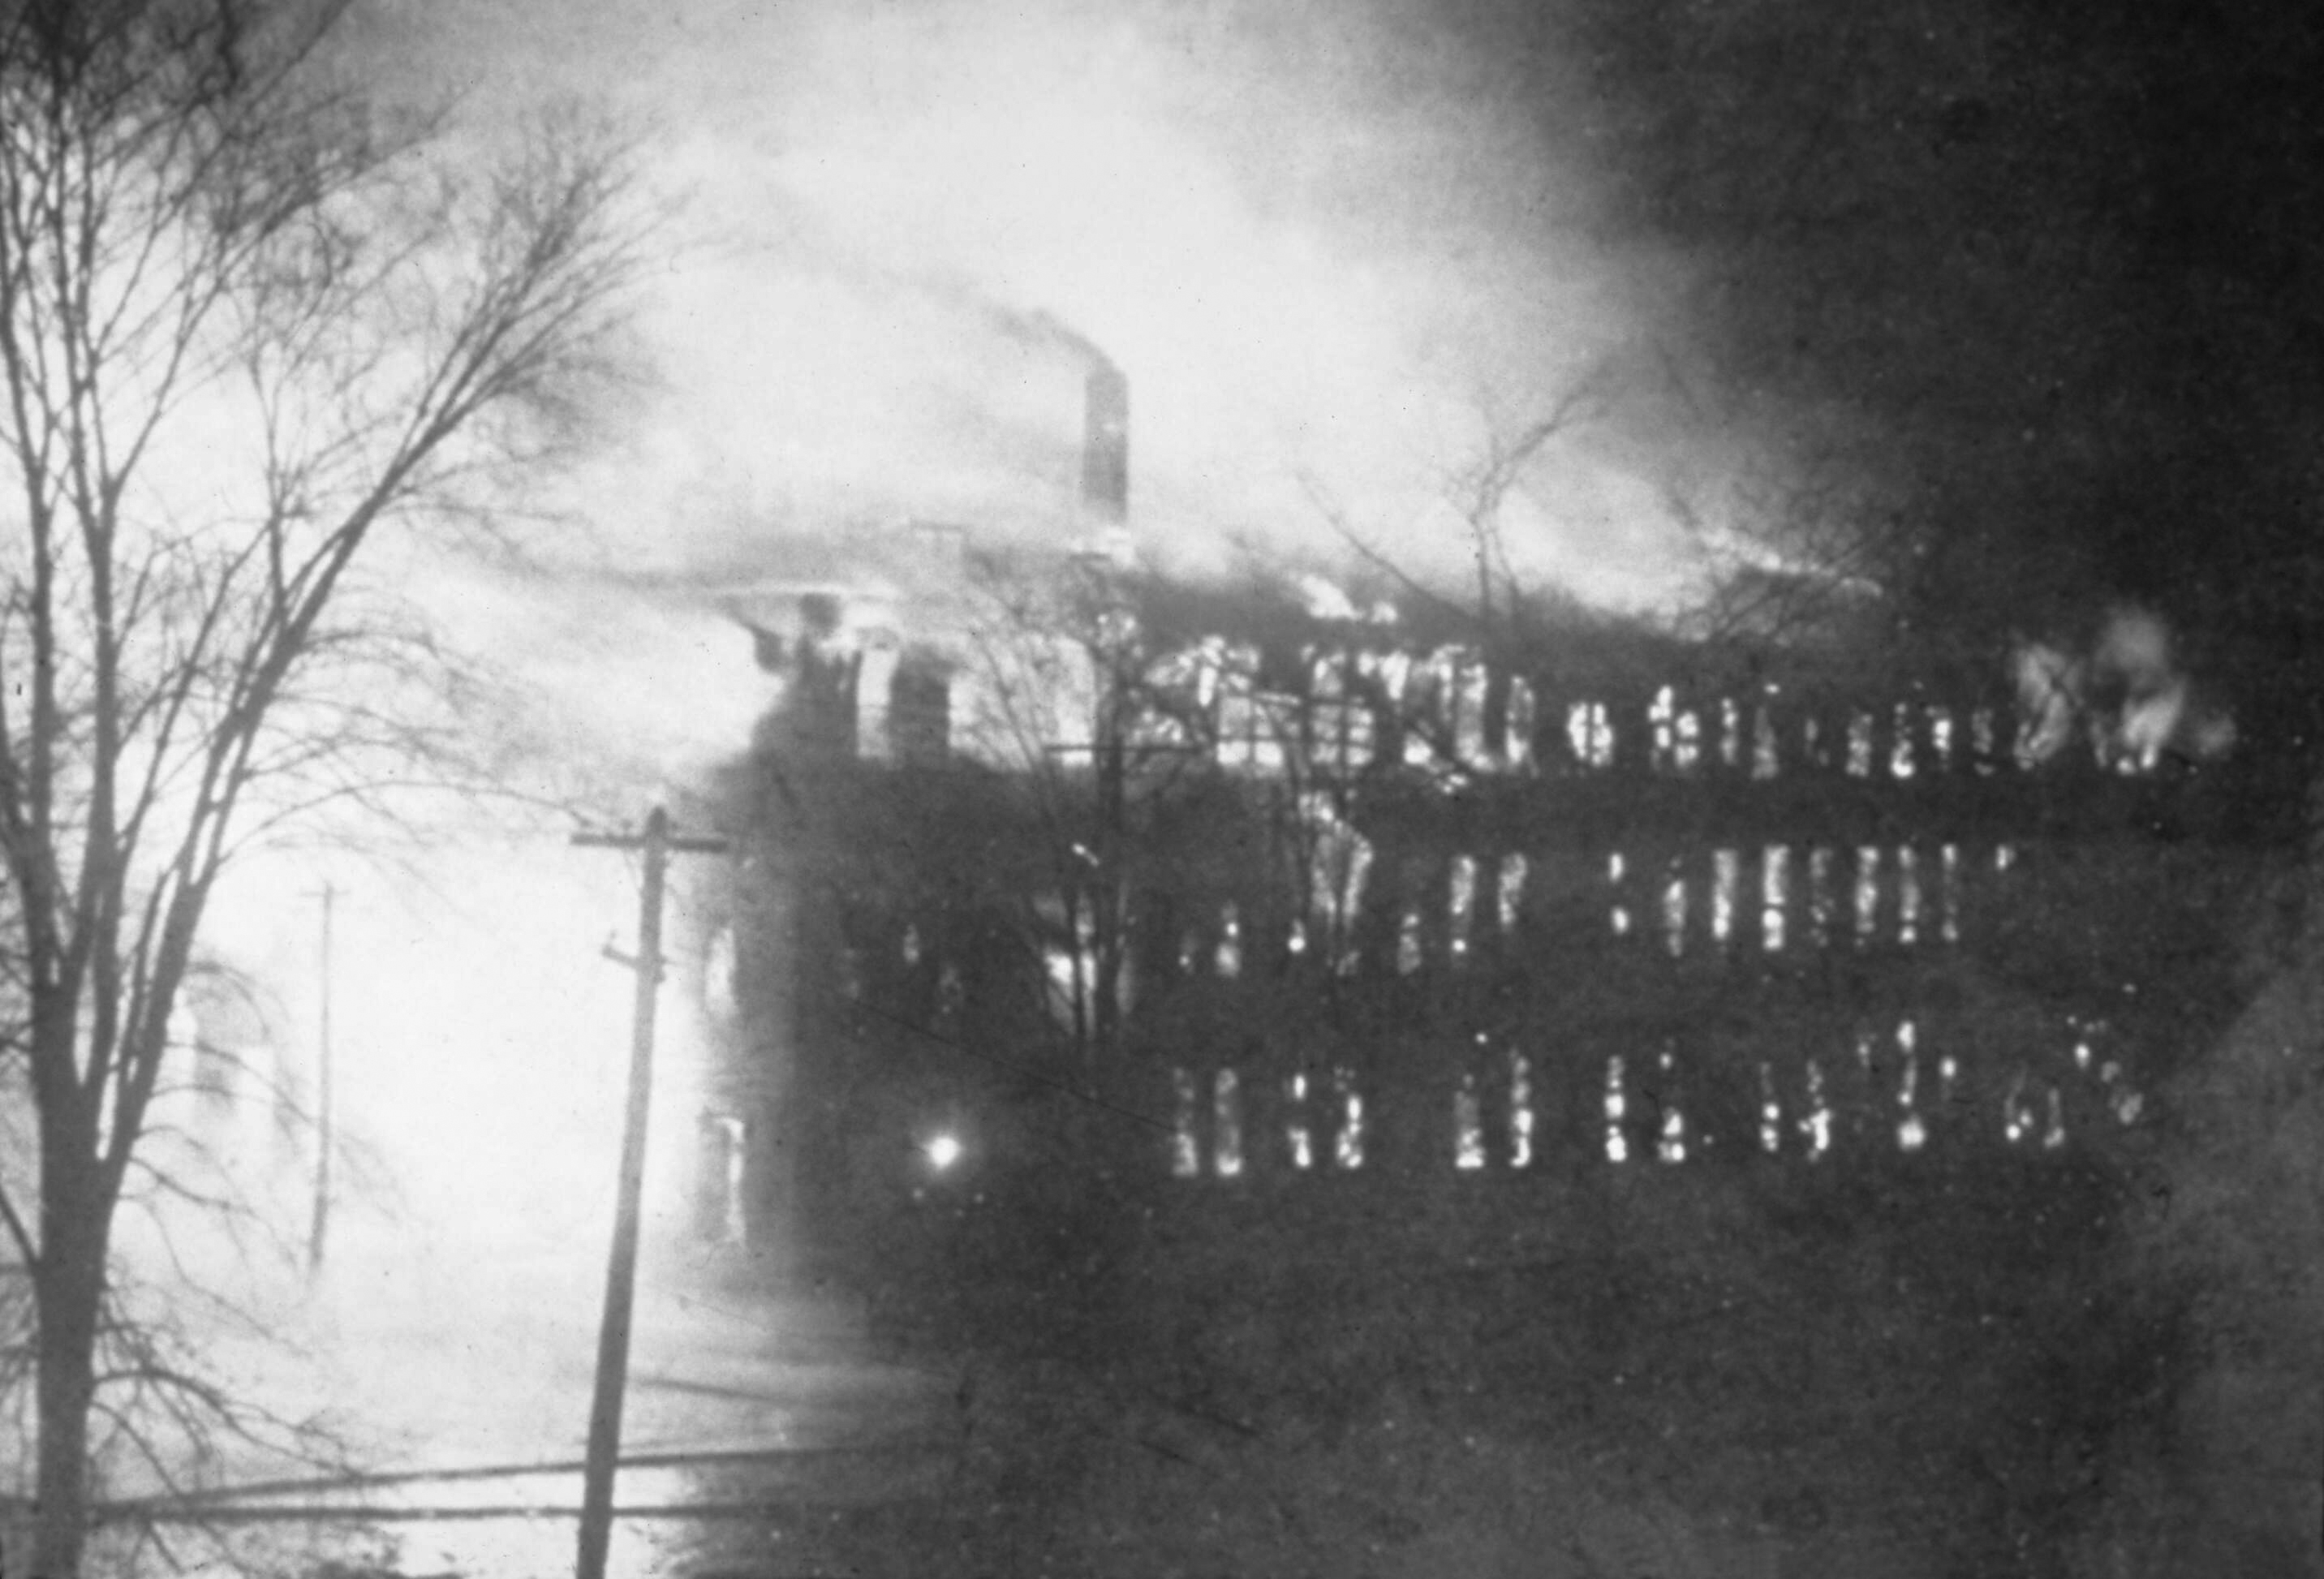
\includegraphics[width=1\linewidth]{images/review-and-herlad.jpg}
    \caption*{Burning of Review and Herald press building, December 30, 1902.}
    \label{fig:review-and-herald}
\end{figure}


\begin{figure}[h]
    \centering
    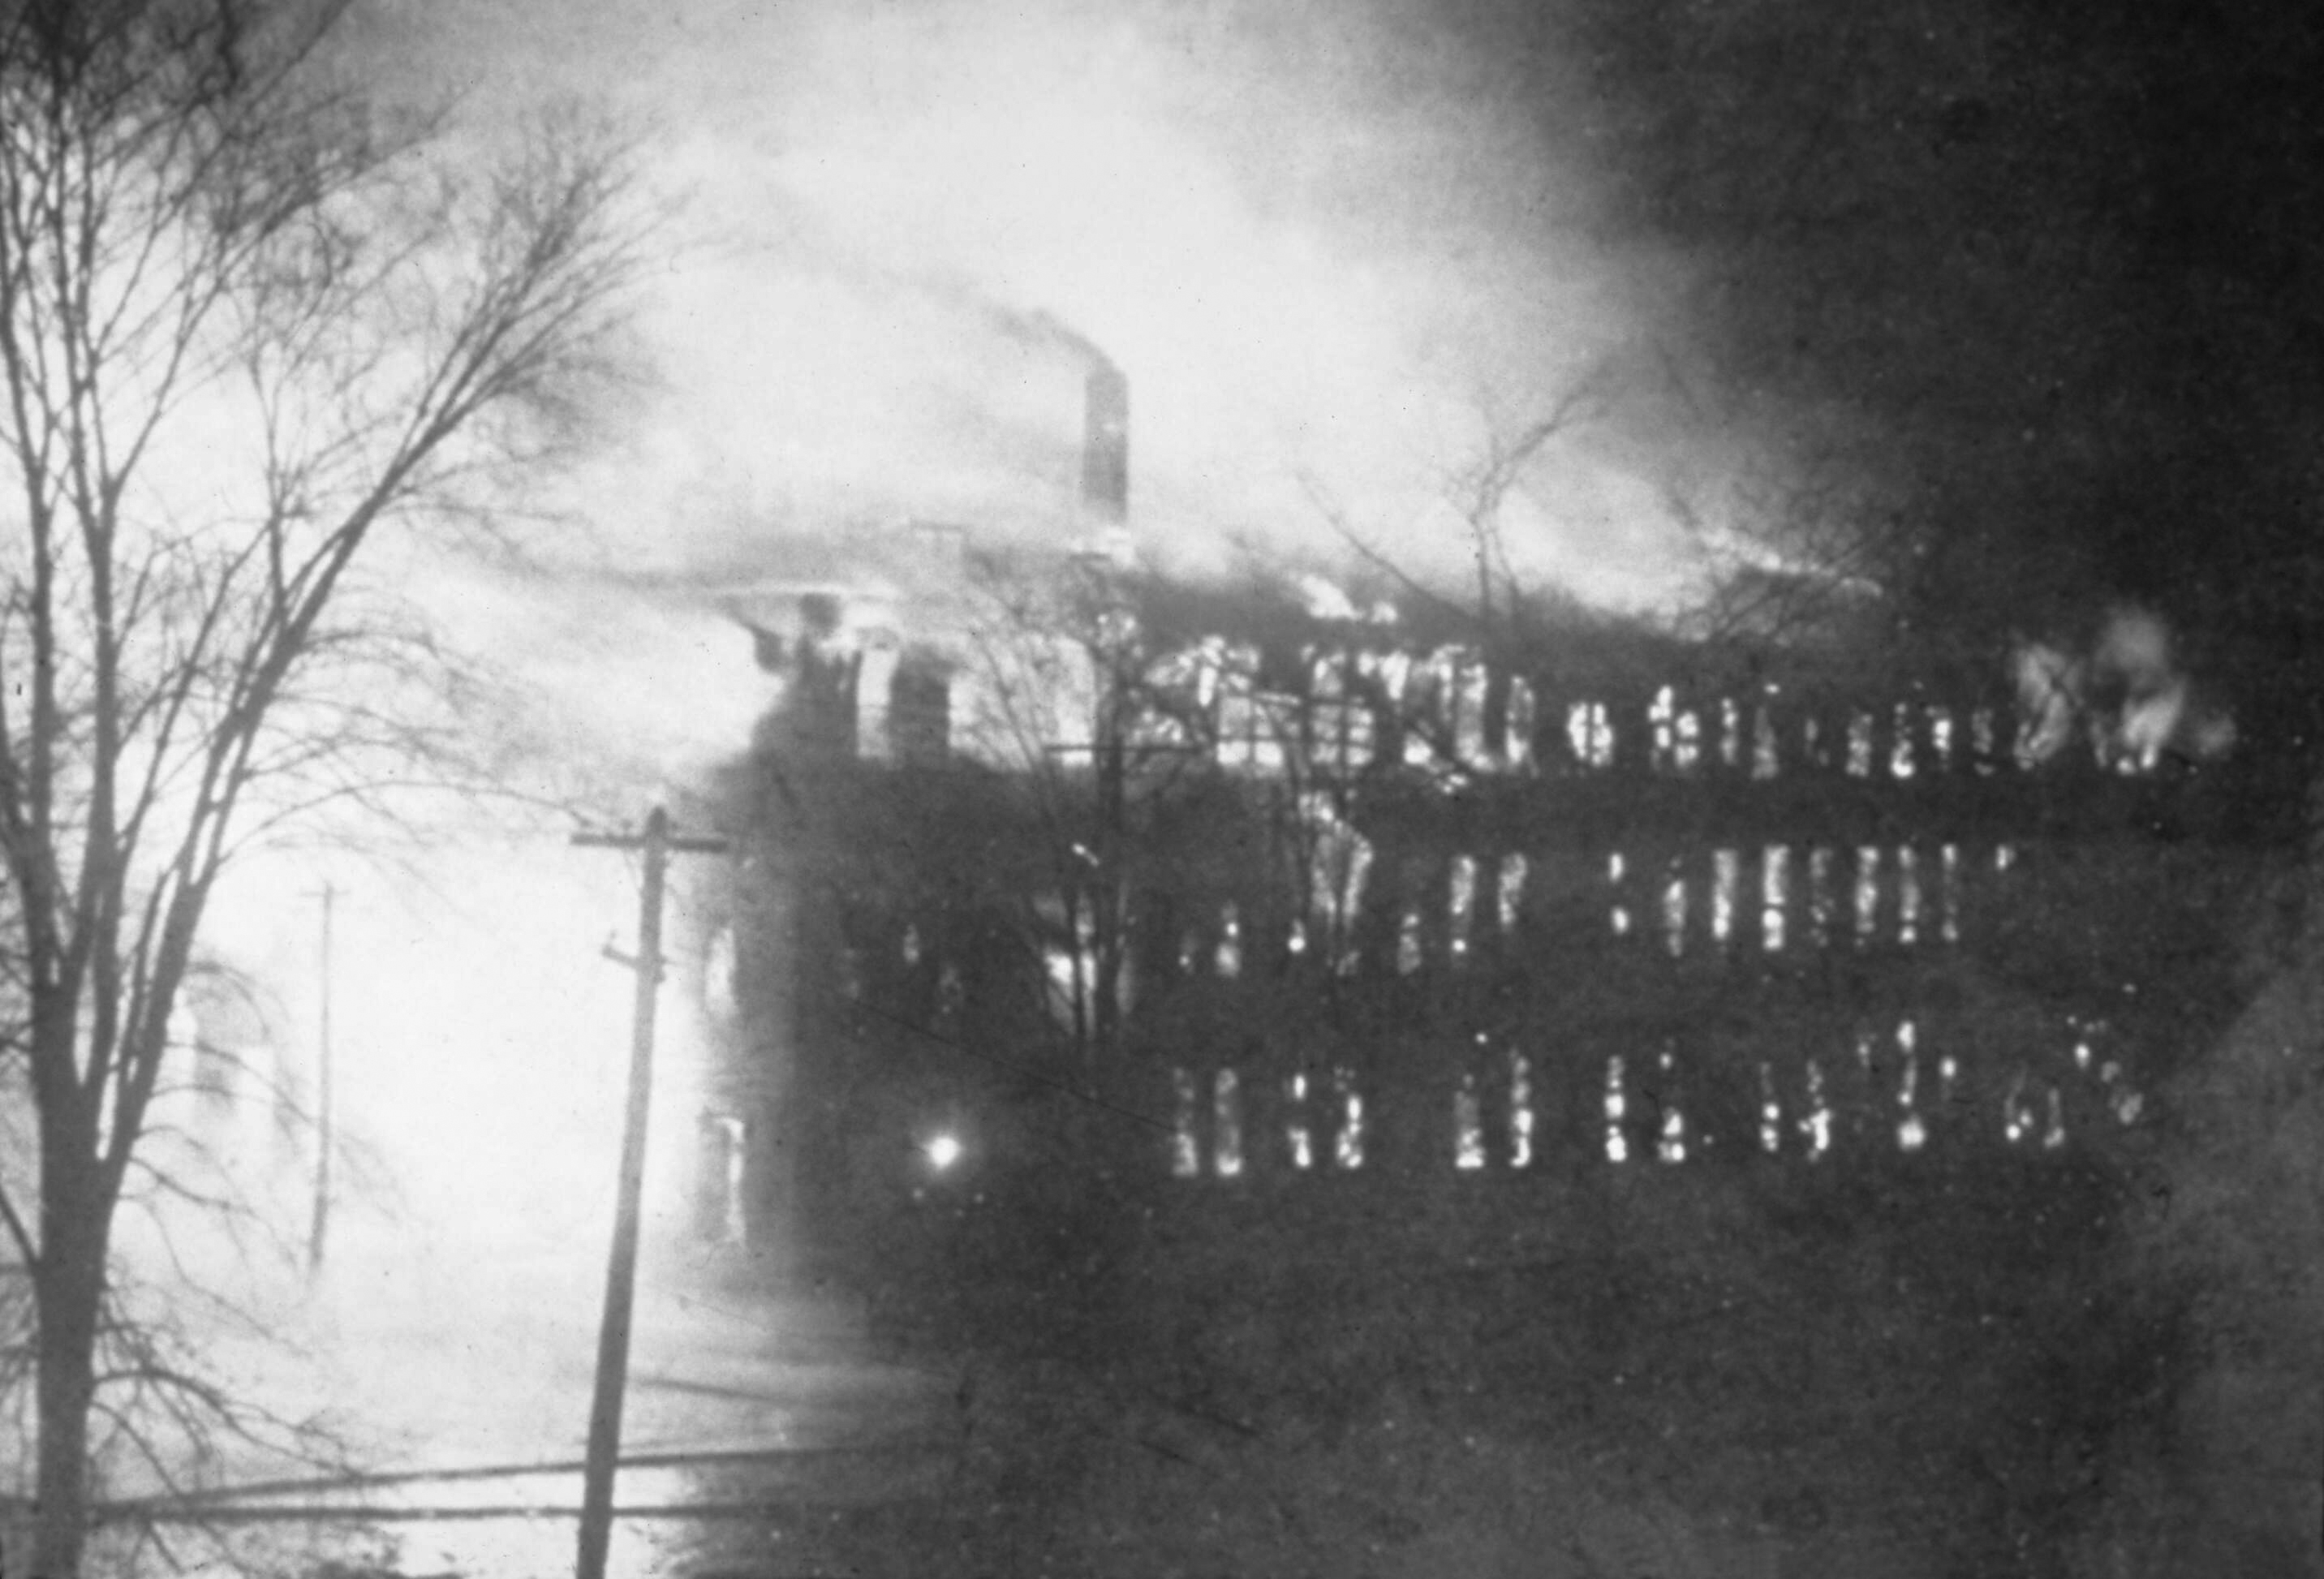
\includegraphics[width=1\linewidth]{images/review-and-herlad.jpg}
    \caption*{Incendie du bâtiment de la presse Review and Herald, 30 décembre 1902.}
    \label{fig:review-and-herald}
\end{figure}


\egw{I have some things to say to our teachers in reference to \textbf{the new book The Living Temple}. \textbf{Be careful how you sustain \underline{the sentiments of this book regarding the personality of God}}. As the Lord presents matters to me, \textbf{these sentiments do not bear the endorsement of God}. \textbf{They are a snare that the enemy has prepared for these last days}. I thought that this would surely be discerned and that it would not be necessary for me to say anything about it. \textbf{But since the claim has been made that the teachings of this book can be sustained by statements from my writings, I am compelled to speak in denial of this claim}. There may be in this book expressions and sentiments that are in harmony with my writings. And there may be in my writings many statements which when taken from their connection, and interpreted according to the mind of the writer of Living Temple, would seem to be in harmony with the teachings of this book. \textbf{This may give apparent support to the assertion that the sentiments in Living Temple are in harmony with my writings}. \textbf{But God forbid that this opinion should prevail}.}[Lt211-1903.1; 1903][https://egwwritings.org/read?panels=p14068.9598008]


\egw{J'ai quelques mots à dire à nos enseignants concernant \textbf{le nouveau livre Le Temple Vivant}. \textbf{Soyez prudents quant à la façon dont vous soutenez \underline{le raisonnement de ce livre concernant la personnalité de Dieu}}. Selon ce que le Seigneur me présente, \textbf{ce raisonnement ne porte pas l'approbation de Dieu}. \textbf{C'est un piège que l'ennemi a préparé pour ces derniers jours}. Je pensais que cela serait sûrement discerné et qu'il ne serait pas nécessaire pour moi de dire quoi que ce soit à ce sujet. \textbf{Mais puisqu'on a prétendu que les enseignements de ce livre peuvent être soutenus par des déclarations de mes écrits, je suis obligée de parler pour nier cette affirmation}. Il peut y avoir dans ce livre des expressions et des sentiments qui sont en harmonie avec mes écrits. Et il peut y avoir dans mes écrits de nombreuses déclarations qui, sorties de leur contexte et interprétées selon l'esprit de l'auteur du Temple Vivant, sembleraient être en harmonie avec les enseignements de ce livre. \textbf{Cela peut donner un soutien apparent à l'affirmation que le raisonnement du Temple Vivant est en harmonie avec mes écrits}. \textbf{Mais que Dieu nous préserve que cette opinion prévale}.}[Lt211-1903.1; 1903][https://egwwritings.org/read?panels=p14068.9598008]


Repeatedly, Sister White stated that the true problem of the book was the sentiments\egwinline{\textbf{regarding the personality of God}}. These sentiments are not sustained by statements from Ellen White's writings and these very sentiments\egwinline{\textbf{are a snare that the enemy has prepared for these last days}}.


À plusieurs reprises, Sœur White a déclaré que le véritable problème du livre était le raisonnement\egwinline{\textbf{concernant la personnalité de Dieu}}. Ce raisonnement n'est pas soutenu par des déclarations des écrits d'Ellen White et ce même raisonnement\egwinline{\textbf{est un piège que l'ennemi a préparé pour ces derniers jours}}.


God, again in His providence, solved this conflict. Kellogg accepted the reproof from the Lord's messenger and, before the council closed, he stated that the Living Temple would be taken from the market\footnote{\href{https://forgottenpillar.com/wp-content/uploads/2022/04/Letter-A-G-Daniells-to-W-C-White-October-29-1903.pdf}{Letter: A. G. Daniells to W. C. White, October 23, 1903, pp. 5}}. But after the conference, he spoke privately with the general conference president, Brother Arthur G. Daniells, about his plans for revising the book. The following is a look at select letters, revealing Kellogg's plans for revising “\textit{Living Temple}”.


Dieu, encore une fois dans Sa providence, a résolu ce conflit. Kellogg a accepté la réprimande de la messagère du Seigneur et, avant la clôture du conseil, il a déclaré que le Temple Vivant serait retiré du marché\footnote{\href{https://forgottenpillar.com/wp-content/uploads/2022/04/Letter-A-G-Daniells-to-W-C-White-October-29-1903.pdf}{Lettre: A. G. Daniells à W. C. White, 23 octobre 1903, pp. 5}}. Mais après la conférence, il s'est entretenu en privé avec le président de la conférence générale, Frère Arthur G. Daniells, au sujet de ses projets de révision du livre. Voici un aperçu de lettres sélectionnées, révélant les plans de Kellogg pour réviser “\textit{Le Temple Vivant}”.


Ellen White was not present at the yearly conference in Washington DC but her son, William C. White, did attend. When the conference was over, brother Arthur G. Daniells wrote a confidential letter to William C. White regarding Dr. Kellogg's plan to revise his book:


Ellen White n'était pas présente à la conférence annuelle à Washington DC, mais son fils, William C. White, y a assisté. Lorsque la conférence s'est terminée, frère Arthur G. Daniells a écrit une lettre confidentielle à William C. White concernant le plan du Dr Kellogg pour réviser son livre:


\others{October 29, 1903}


\others{29 octobre 1903}


\othersnogap{Ever since the \textbf{council closed} I have felt that I should write you \textbf{confidentially regarding Dr. Kellogg's plans for revising and republishing ‘The Living Temple’}…. He \normaltext{[Kellogg]} said that some days before coming to the council, he had been thinking the matter over, and began to see that \textbf{he had made a slight mistake in expressing his views}. He said that all the way along he had been troubled to know how to state the character of God and his relation to his creation works…}


\othersnogap{Depuis que \textbf{le conseil s'est terminé}, j'ai senti que je devrais vous écrire \textbf{confidentiellement concernant les plans du Dr Kellogg pour réviser et republier ‘Le Temple Vivant’}... Il \normaltext{[Kellogg]} a dit que quelques jours avant de venir au conseil, il avait réfléchi à la question et avait commencé à voir qu’\textbf{il avait fait une légère erreur en exprimant ses vues}. Il a dit que tout au long du chemin, il avait été troublé de savoir comment décrire le caractère de Dieu et sa relation avec ses œuvres de création...}


\begin{figure}[hp]
    \centering
    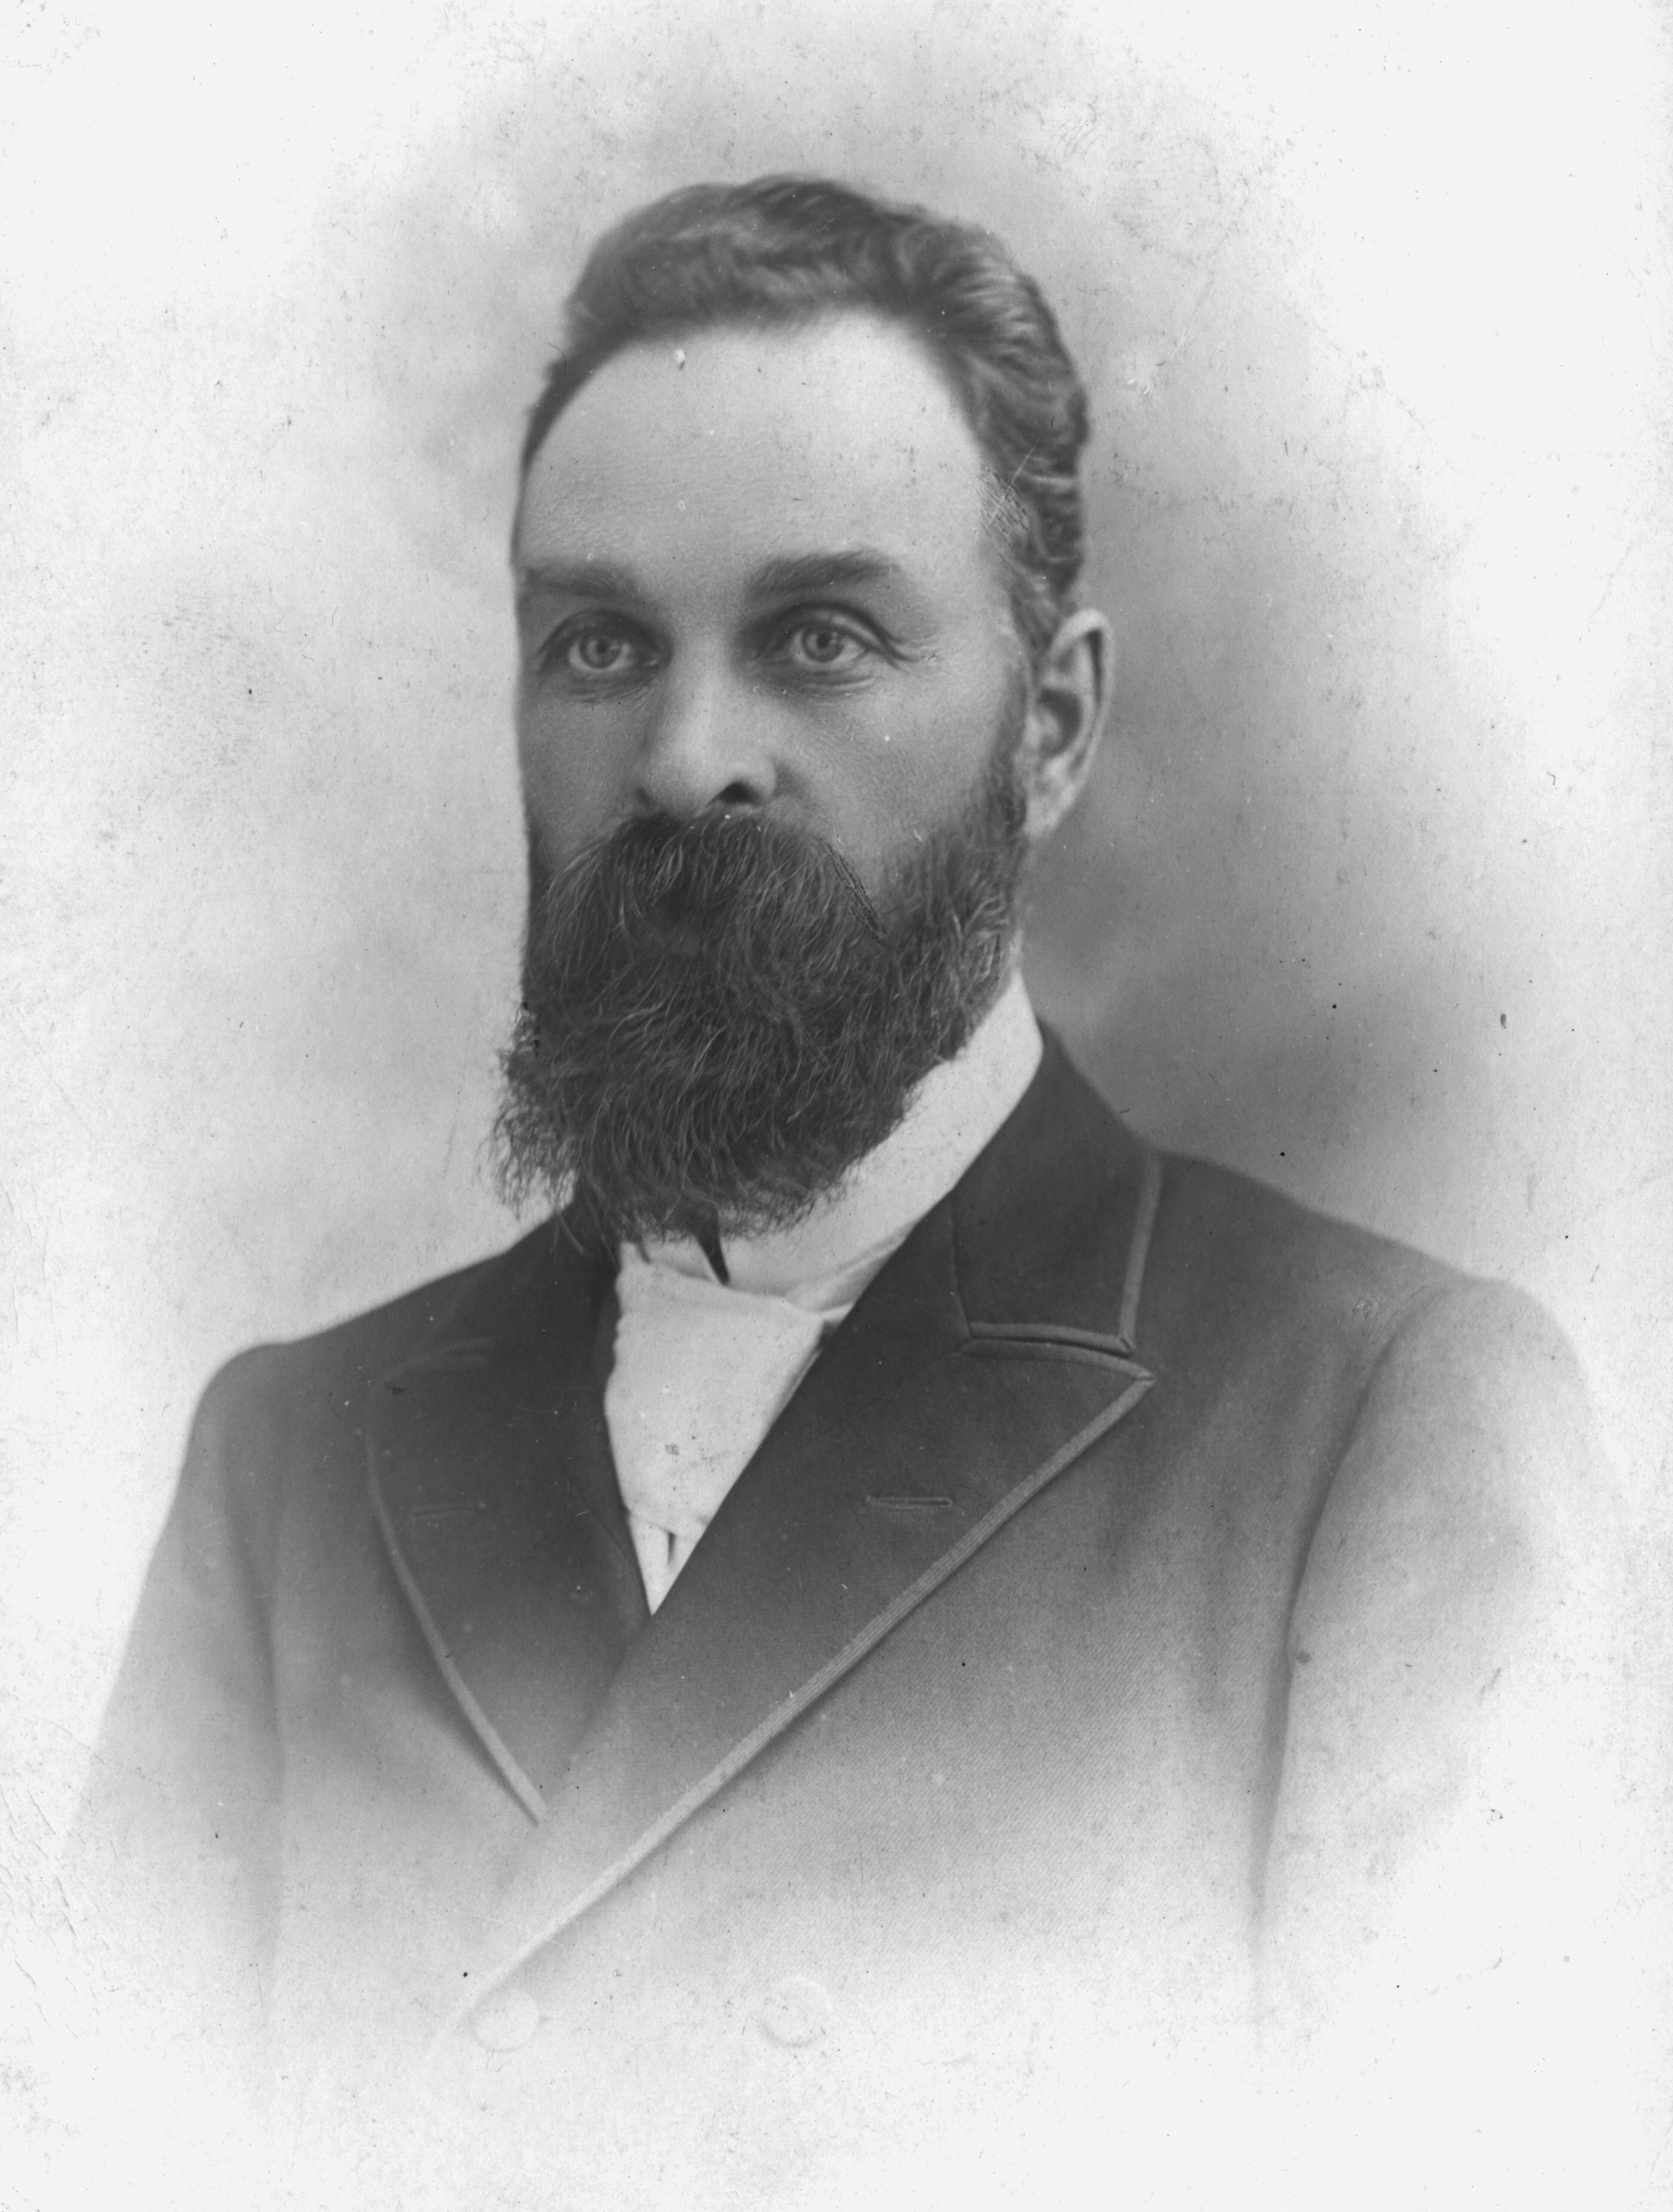
\includegraphics[width=1\linewidth]{images/daniels.jpg}
    \caption*{Arthur Grosvenor Daniells (1858-1935)}
    \label{fig:daniells}
\end{figure}


\begin{figure}[hp]
    \centering
    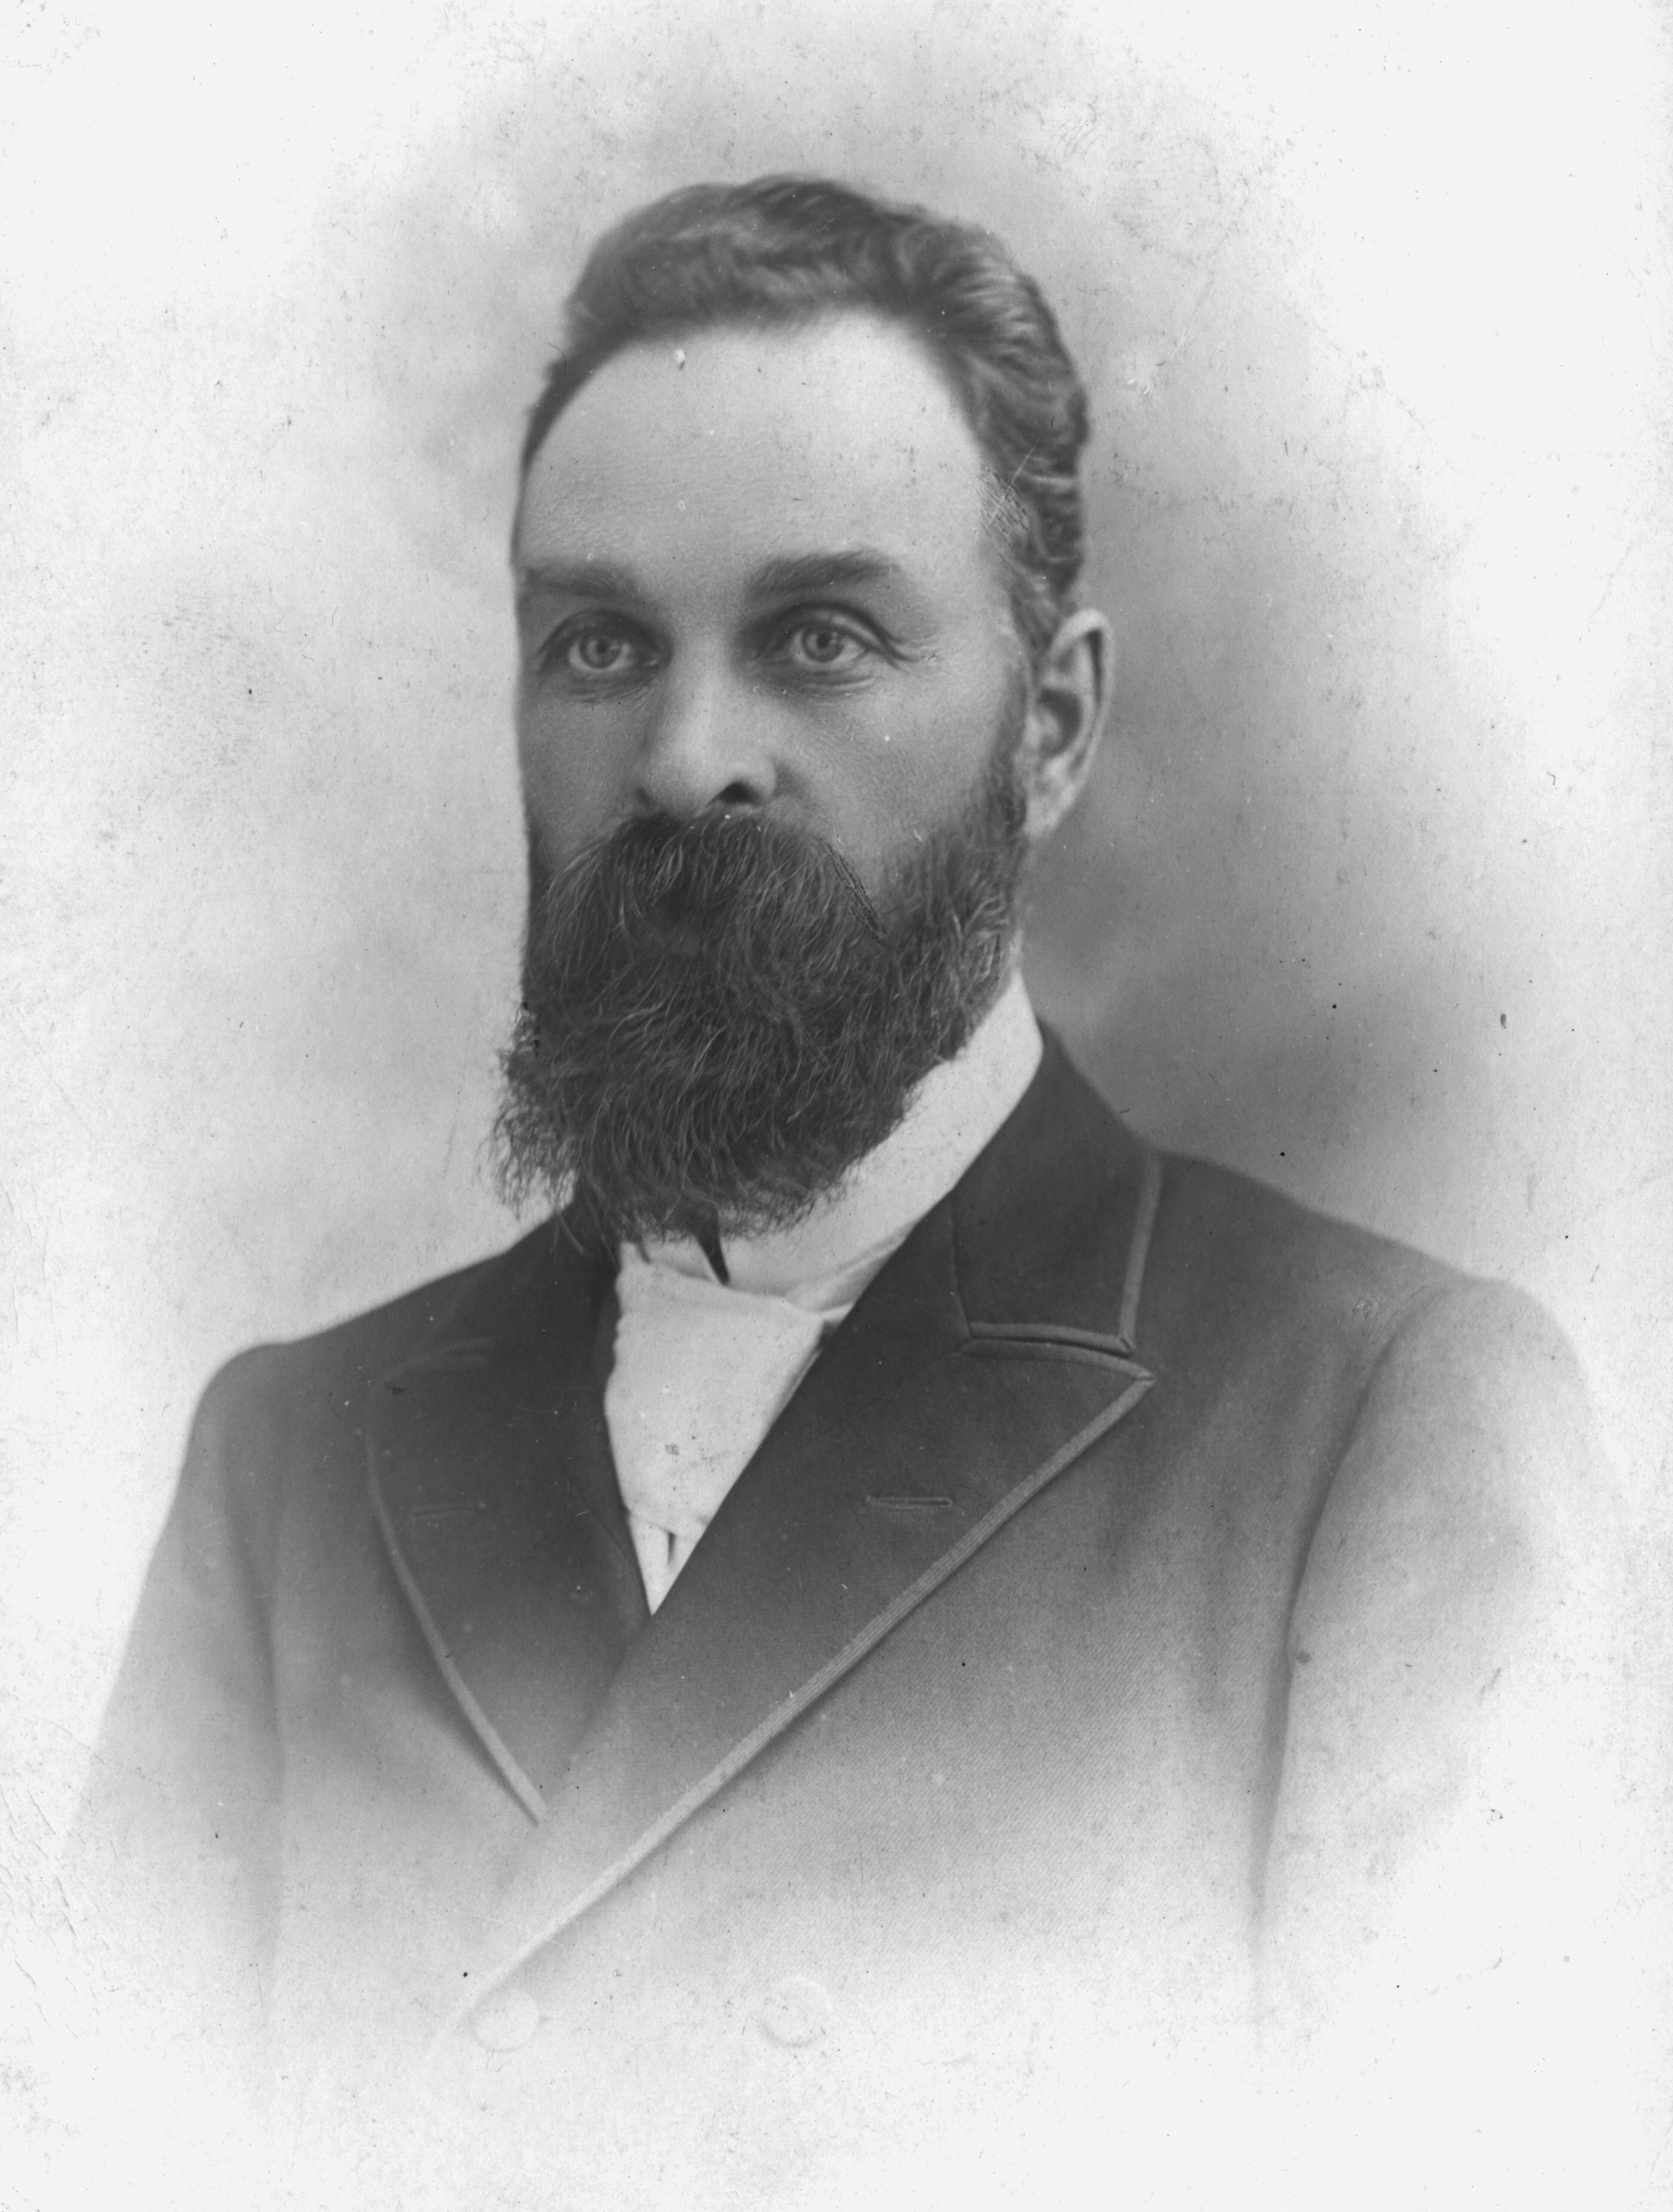
\includegraphics[width=1\linewidth]{images/daniels.jpg}
    \caption*{Arthur Grosvenor Daniells (1858-1935)}
    \label{fig:daniells}
\end{figure}


\othersnogap{\textbf{He then stated that his former views \underline{regarding the trinity} had stood in his way of making a clear and absolutely correct statement; but that within a short time \underline{he had come to believe in the trinity} and could now see pretty clearly where all the difficulty was, and believed that he could clear the matter up satisfactorily.}}


\othersnogap{\textbf{Il a ensuite déclaré que ses opinions antérieures \underline{concernant la trinité} l'avaient empêché de faire une déclaration claire et absolument correcte ; mais qu'en peu de temps \underline{il en était venu à croire en la trinité} et qu'il pouvait maintenant voir assez clairement où se situait toute la difficulté, et qu'il croyait pouvoir clarifier la question de manière satisfaisante.}}


\othersnogap{\textbf{He told me that he now believed in \underline{God the Father, God the Son, and God the Holy Ghost}; and his view was that it was God the Holy Ghost, and not God the Father, that filled all space, and every living thing. He said if he had believed \underline{this} before writing the book, he could have expressed his views without giving the wrong impression the book now gives.}}


\othersnogap{\textbf{Il m'a dit qu'il croyait maintenant en \underline{Dieu le Père, Dieu le Fils et Dieu le Saint-Esprit} ; et selon lui, c'était Dieu le Saint-Esprit, et non Dieu le Père, qui remplissait tout l'espace et chaque être vivant. Il a dit que s'il avait cru \underline{cela} avant d'écrire le livre, il aurait pu exprimer ses opinions sans donner la mauvaise impression que donne maintenant le livre.}}


\othersnogap{\textbf{I placed before him the objections I found in the teaching, and tried to show him that the teaching was so utterly contrary to the gospel that I did not see how it could be revised by changing a few expressions.}}


\othersnogap{\textbf{J'ai exposé devant lui les objections que j'ai trouvées dans l'enseignement, et j'ai essayé de lui montrer que cet enseignement était si totalement contraire à l'évangile que je ne voyais pas comment il pourrait être révisé en changeant quelques expressions.}}


\othersnogap{We argued the matter at some length in a friendly way; but I felt sure that when we parted, the doctor did not understand himself, nor the character of his teaching. And I could not see how it would be possible for him to flop over, \textbf{and in the course of a few days \underline{fix the books up} so that it would be all right}.}[Letter: A. G. Daniells to W. C. White, October 29, 1903. pp. 1, 2][https://forgotten-pillar.s3.us-east-2.amazonaws.com/Letter-A-G-Daniells-to-W-C-White-October-29-1903.pdf]


\othersnogap{Nous avons discuté de la question assez longuement de manière amicale ; mais j'étais certain qu'en nous séparant, le docteur ne se comprenait pas lui-même, ni le caractère de son enseignement. Et je ne voyais pas comment il lui serait possible de changer d'avis, \textbf{et en l'espace de quelques jours \underline{arranger les livres} pour que tout soit en ordre}.}[Letter: A. G. Daniells to W. C. White, October 29, 1903. pp. 1, 2][https://forgotten-pillar.s3.us-east-2.amazonaws.com/Letter-A-G-Daniells-to-W-C-White-October-29-1903.pdf]


Kellogg did not see the mistake in his sentiments; but rather, in expressing his views. He did not think that his views were false, merely his expression of those views, which led to the book giving a wrong impression. Yet, evidently, this was not true. As Sister White had stated, Kellogg had a problem with the sentiments regarding the \emcap{personality of God} and where His presence is. So, Kellogg suggested that in order to “\textit{fix the books up}” he would include the trinitarian expressions because he now started to believe in \textit{the Trinity} doctrine. At this point in time, the Seventh-day Adventist Church was not trinitarian—the doctrine of Trinity was not part of the \emcap{Fundamental Principles}, as we saw previously. Thus, it is no surprise that Brother Daniels objected and refuted Trinitarian teaching, claiming that it was\others{so utterly contrary to the gospel.} Revising the book, by changing a few expressions, would not change the main problem of the book: the sentiments on the \emcap{personality of God}.


Kellogg ne voyait pas l'erreur dans son raisonnement ; mais plutôt, dans l'expression de ses opinions. Il ne pensait pas que ses opinions étaient fausses, simplement son expression de ces opinions, ce qui avait conduit le livre à donner une mauvaise impression. Pourtant, manifestement, ce n'était pas vrai. Comme Sœur White l'avait déclaré, Kellogg avait un problème avec le raisonnement concernant la \emcap{personnalité de Dieu} et où se trouve Sa présence. Ainsi, Kellogg a suggéré que pour “\textit{arranger les livres}” il inclurait les expressions trinitaires parce qu'il commençait maintenant à croire en \textit{la doctrine de la Trinité}. À cette époque, l'Église Adventiste du Septième Jour n'était pas trinitaire—la doctrine de la Trinité ne faisait pas partie des \emcap{Principes Fondamentaux}, comme nous l'avons vu précédemment. Il n'est donc pas surprenant que Frère Daniels ait objecté et réfuté l'enseignement trinitaire, affirmant qu'il était\others{si totalement contraire à l'évangile.} Réviser le livre, en changeant quelques expressions, ne changerait pas le problème principal du livre : le raisonnement sur la \emcap{personnalité de Dieu}.


In the described events, and in William White's response to Brother Daniells, we can see why Sister White wrote the Special Testimonies. William White responded to Brother Daniells on Nov. 4, 1903:


Dans les événements décrits, et dans la réponse de William White au Frère Daniells, nous pouvons voir pourquoi Sœur White a écrit les Témoignages Spéciaux. William White a répondu au Frère Daniells le 4 novembre 1903 :


\others{Dear Brother, --}


\others{Cher Frère, --}


\othersnogap{\textbf{\underline{Mother and I} have just read your letter of \underline{October 29} in which you speak of the \underline{various plans that have been proposed for the revising and reproduction of ‘The Living Temple}.’}}


\othersnogap{\textbf{\underline{Mère et moi} venons de lire votre lettre du \underline{29 octobre} dans laquelle vous parlez des \underline{divers plans qui ont été proposés pour la révision et la reproduction du ‘Temple Vivant (le livre)}’.}}


\othersnogap{We were pleasantly surprised at the announcement that Dr. Kellogg would withdraw this book from the market, \textbf{and we are sorry indeed that his mind is swinging back to the plan of revising it, \underline{Mother expresses herself quite emphatically regarding this matter; she regards it as an unprofitable undertaking}}. I think she will write to you soon expressing her views regarding this.}


\othersnogap{Nous avons été agréablement surpris par l'annonce que le Dr Kellogg retirerait ce livre du marché, \textbf{et nous sommes vraiment désolés que son esprit revienne au plan de le réviser, \underline{Mère s'exprime assez catégoriquement concernant cette question ; elle considère cela comme une entreprise improductive}}. Je pense qu'elle vous écrira bientôt pour exprimer son point de vue à ce sujet.}


\othersnogap{\textbf{… I believe it will be necessary \underline{to issue a special Testimony soon}, and this must contain a very full and clear statement on the positive side of this question, as well as articles pointing out the errors in the teaching of those who have departed from the truth through fascinating and deceptive theories}.}[\href{https://ellenwhite.org/letterbooks/555}{Letter from W.C. White to A.G. Daniells, Nov. 4, 1903,} (p. 458)]


\othersnogap{\textbf{… Je crois qu'il sera nécessaire \underline{de publier bientôt un Témoignage spécial}, et celui-ci doit contenir une déclaration très complète et claire sur le côté positif de cette question, ainsi que des articles soulignant les erreurs dans l'enseignement de ceux qui se sont écartés de la vérité à travers des théories fascinantes et trompeuses}.}[\href{https://ellenwhite.org/letterbooks/555}{Lettre de W.C. White à A.G. Daniells, 4 nov. 1903,} (p. 458)]


\begin{figure}[h]
    \centering
    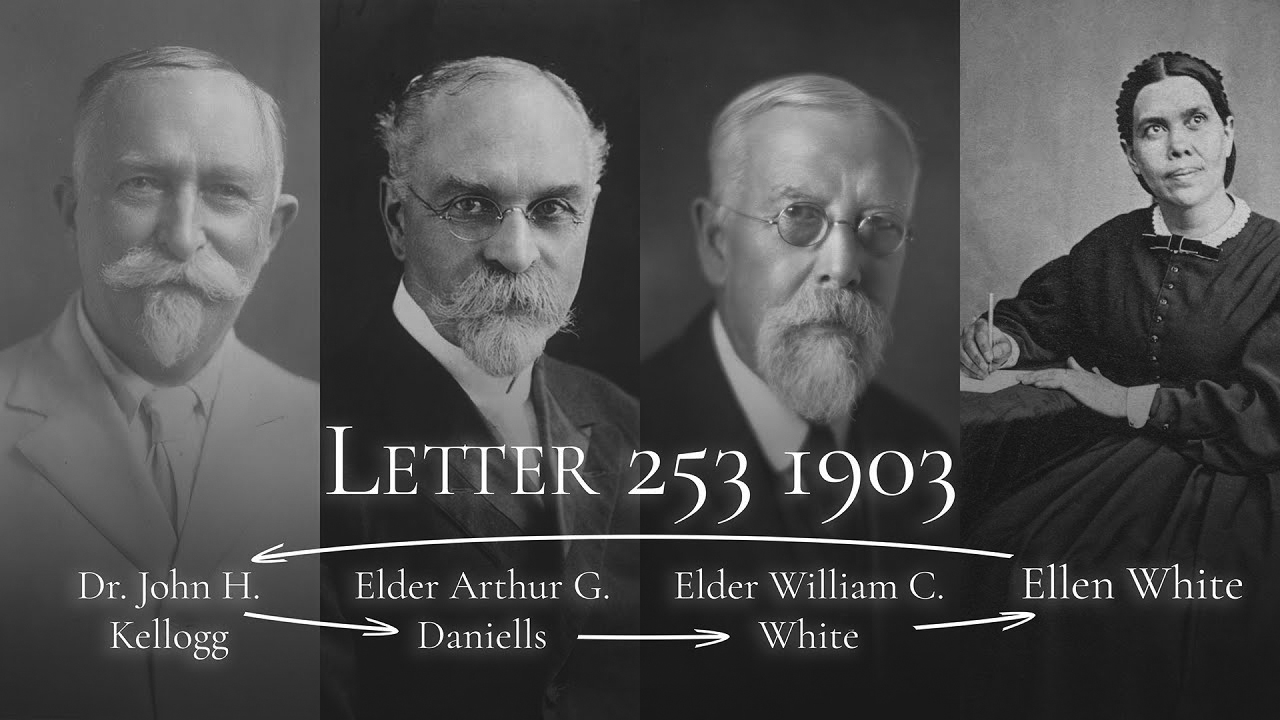
\includegraphics[width=1\linewidth]{images/correspondance.jpg}
    \caption*{Correspondence chain between A. G. Daniells, W. C. White, Ellen White and Dr. John H. Kellogg.}
    \label{fig:corespondance}
\end{figure}


\begin{figure}[h]
    \centering
    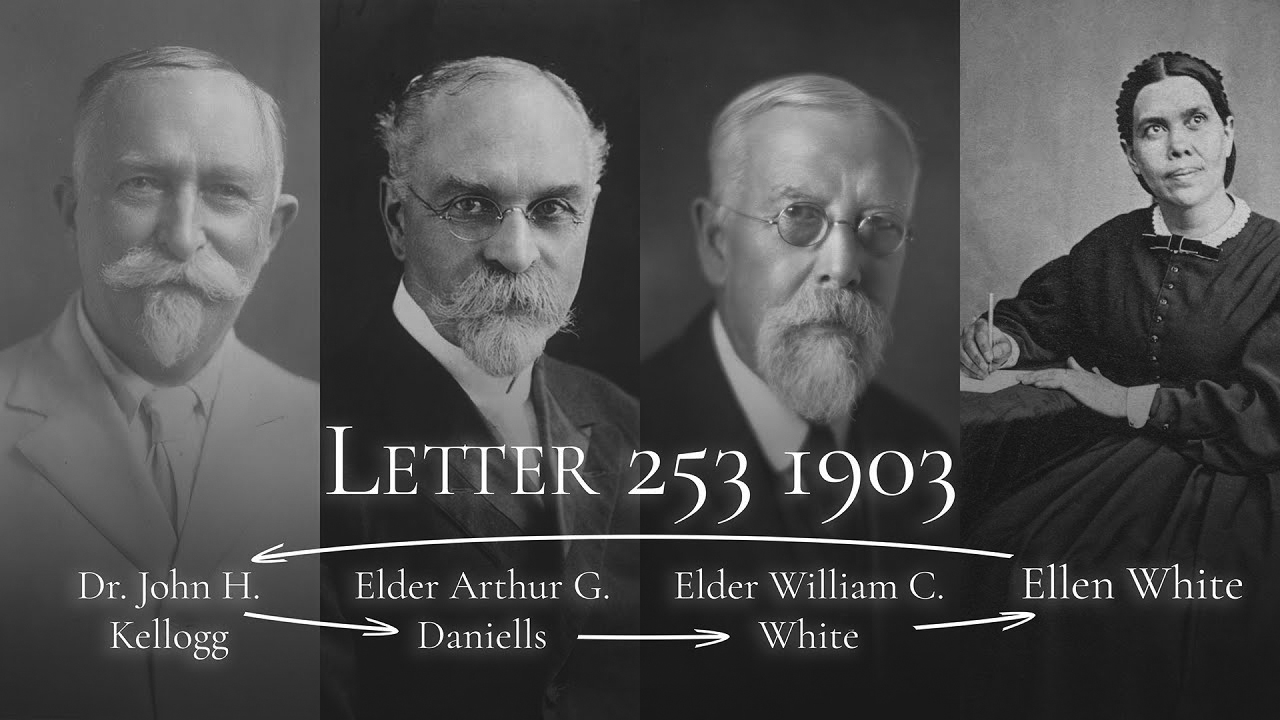
\includegraphics[width=1\linewidth]{images/correspondance.jpg}
    \caption*{Chaîne de correspondance entre A. G. Daniells, W. C. White, Ellen White et Dr. John H. Kellogg.}
    \label{fig:corespondance}
\end{figure}


Here is evidence that Sister White was familiar with Dr. Kellogg's intentions to revise “\textit{Living Temple}” and her familiarity with his belief in the Trinity doctrine. In William's words, she expressed herself quite emphatically regarding this matter. She deemed it an unprofitable undertaking. For this reason, it was necessary to issue a special Testimony soon. And there it was. This is how the \textit{Testimonies for the Church Containing Letters to Physicians and Ministers Instruction to Seventh-Day Adventists} was published in 1904, containing letters to the physicians and ministers connected to Kellogg's crisis.


Voici la preuve que Sœur White connaissait les intentions du Dr. Kellogg de réviser “\textit{Le Temple Vivant (le livre)}” et sa familiarité avec sa croyance en la doctrine de la Trinité. Selon les mots de William, elle s'est exprimée de manière assez catégorique sur cette question. Elle l'a jugée comme une entreprise non profitable. Pour cette raison, il était nécessaire de publier bientôt un Témoignage spécial. Et c'est ce qui s'est produit. C'est ainsi que les \textit{Témoignages pour l'Église contenant des lettres aux médecins et aux pasteurs - Instruction aux Adventistes du Septième Jour} ont été publiés en 1904, contenant des lettres aux médecins et aux pasteurs liés à la crise de Kellogg.


By saying \others{\textbf{\underline{Mother and I} have just read your letter of \underline{October 29}}}, William testified that Sister White was fully aware of Kellogg's intentions and trinitarian belief. After she read Daniells’ letter, she wrote a direct reply to Dr. Kellogg. This letter is \textit{Lt253-1903}. It is a very prominent and eye opening letter because it clearly exposes how the prophet dealt with the Trinity doctrine. She elevated the doctrine on the \emcap{personality of God} constituted in the \emcap{Fundamental Principles}. There are striking similarities between this letter and the tenth chapter of the Special Testimonies, \textit{The Foundation of our Faith}.


En disant \others{\textbf{\underline{Mère et moi} venons de lire votre lettre du \underline{29 octobre}}}, William a témoigné que Sœur White était pleinement consciente des intentions de Kellogg et de sa croyance trinitaire. Après avoir lu la lettre de Daniells, elle a écrit une réponse directe au Dr. Kellogg. Cette lettre est \textit{Lt253-1903}. C'est une lettre très importante et révélatrice car elle expose clairement comment la prophétesse a traité la doctrine de la Trinité. Elle a élevé la doctrine sur la \emcap{personnalité de Dieu} constituée dans les \emcap{principes fondamentaux}. Il y a des similitudes frappantes entre cette lettre et le dixième chapitre des Témoignages Spéciaux, \textit{Le Fondement de notre Foi}.


% Revision of the Living Temple

\begin{titledpoem}
    
    \stanza{
        In Kellogg’s book, a subtle snare \\
        Though well-disguised through crafty care \\
        From Bible truth would lead away \\
        And cause some precious souls to stray.
    }

    \stanza{
        And though much scripture there was used \\
        The early truth became confused \\
        This error served to twist the mind \\
        But in God’s Word the truth we find.
    }

    \stanza{
        God’s personality has form \\
        To Bible truth we must conform \\
        On this the Doctor wasn’t clear \\
        But early Advent truth is dear
    }
    
\end{titledpoem}